\PassOptionsToPackage{unicode=true}{hyperref} % options for packages loaded elsewhere
\PassOptionsToPackage{hyphens}{url}
%
\documentclass[
]{article}
\usepackage{lmodern}
\usepackage{amssymb,amsmath}
\usepackage{ifxetex,ifluatex}
\ifnum 0\ifxetex 1\fi\ifluatex 1\fi=0 % if pdftex
  \usepackage[T1]{fontenc}
  \usepackage[utf8]{inputenc}
  \usepackage{textcomp} % provides euro and other symbols
\else % if luatex or xelatex
  \usepackage{unicode-math}
  \defaultfontfeatures{Scale=MatchLowercase}
  \defaultfontfeatures[\rmfamily]{Ligatures=TeX,Scale=1}
\fi
% use upquote if available, for straight quotes in verbatim environments
\IfFileExists{upquote.sty}{\usepackage{upquote}}{}
\IfFileExists{microtype.sty}{% use microtype if available
  \usepackage[]{microtype}
  \UseMicrotypeSet[protrusion]{basicmath} % disable protrusion for tt fonts
}{}
\makeatletter
\@ifundefined{KOMAClassName}{% if non-KOMA class
  \IfFileExists{parskip.sty}{%
    \usepackage{parskip}
  }{% else
    \setlength{\parindent}{0pt}
    \setlength{\parskip}{6pt plus 2pt minus 1pt}}
}{% if KOMA class
  \KOMAoptions{parskip=half}}
\makeatother
\usepackage{xcolor}
\IfFileExists{xurl.sty}{\usepackage{xurl}}{} % add URL line breaks if available
\IfFileExists{bookmark.sty}{\usepackage{bookmark}}{\usepackage{hyperref}}
\hypersetup{
  pdfborder={0 0 0},
  breaklinks=true}
\urlstyle{same}  % don't use monospace font for urls
\usepackage[margin=1in]{geometry}
\usepackage{graphicx,grffile}
\makeatletter
\def\maxwidth{\ifdim\Gin@nat@width>\linewidth\linewidth\else\Gin@nat@width\fi}
\def\maxheight{\ifdim\Gin@nat@height>\textheight\textheight\else\Gin@nat@height\fi}
\makeatother
% Scale images if necessary, so that they will not overflow the page
% margins by default, and it is still possible to overwrite the defaults
% using explicit options in \includegraphics[width, height, ...]{}
\setkeys{Gin}{width=\maxwidth,height=\maxheight,keepaspectratio}
\setlength{\emergencystretch}{3em}  % prevent overfull lines
\providecommand{\tightlist}{%
  \setlength{\itemsep}{0pt}\setlength{\parskip}{0pt}}
\setcounter{secnumdepth}{-2}
% Redefines (sub)paragraphs to behave more like sections
\ifx\paragraph\undefined\else
  \let\oldparagraph\paragraph
  \renewcommand{\paragraph}[1]{\oldparagraph{#1}\mbox{}}
\fi
\ifx\subparagraph\undefined\else
  \let\oldsubparagraph\subparagraph
  \renewcommand{\subparagraph}[1]{\oldsubparagraph{#1}\mbox{}}
\fi

% set default figure placement to htbp
\makeatletter
\def\fps@figure{htbp}
\makeatother

\usepackage[french]{babel} \usepackage{hyperref} \usepackage{booktabs} \hypersetup{ colorlinks=true, linkcolor=blue, filecolor=magenta, urlcolor=cyan, }

\author{}
\date{\vspace{-2.5em}}

\begin{document}

\newpage
\begin{flushright}
    \textbf{Équipe 8}
\end{flushright}

\begin{center}
    \vspace{2\baselineskip}
    Charles Comeau \\
    (111 185 421) \\
    \vspace{1\baselineskip}
    Nicholas Langevin \\
    (111 184 631) \\
    \vspace{1\baselineskip}
    Andréanne Larouche \\
    (111 190 518) \\
    \vspace{7\baselineskip}
    Apprentissage statistique en actuariat\\
    ACT-3114 \\
    \vspace{7\baselineskip}
    {\large
    \textbf{Analyse des données de renouvellement d'assurance}} \\
    \vspace{8\baselineskip}
    présenté à \\
    Marie-Pier Côté \\
    \vspace{9\baselineskip}
    École d’actuariat \\
    Université Laval \\
    27 février 2020
\end{center}

\newpage

\tableofcontents

\newpage

\hypertarget{introduction}{%
\section{Introduction}\label{introduction}}

Les données qui seront analysées dans ce rapport proviennent du jeu de
données ``eudirectlapse'' du paquetage ``CASdatasets'' de R. Dans le but
de modéliser le statut de renouvellement d'une police d'assurance,
représenté par la variable ``lapse'' dans ce cas-ci, il sera d'abord
nécessaire de visualiser et de pré-traiter les données observées des 23
060 polices d'assurance. Il est à noter que la durée d'observation est
de un an et que l'année visée et la compagnie demeurent inconnue. On
pourra distincguer les statuts de renouvellement comme étant affiché à
annulé(``Cancellation'') ou à renouvellement (``Renew'') selon le cas
approprié. Ce jeu de données est intéressant du fait qu'il permettera au
fur de l'analyse de nous indiquer les variables types ayant un impact
sur la décision de renouvellement de police des assurés d'une compagnie
d'assurance X. En plus d'être un problème de nature actuarielle, le jeu
de données choisi pourra nous permettre d'entammer une ouverture des
réflexions possibles lorsque nous aurons à travailler dans une compagnie
d'assurance. Étant trois personnes intéressés par l'assurance de
dommages, ce problème nous semblait des plus appropriés et intéressant
face à nos intérêts communs. Le nombre d'observations est également
intéressant car il nous permettera de porter des conclusions précise
avec assez de crédibilité sans toutefois être avoir à travailler avec un
jeu de données inutilement trop volumineux. De plus, chaque variable
explicative semble à prime à bord intéressante pour l'analyse et assez
pertinente, ce que nous pourrons découvrir dans l'élaboration de ce
travail pratique.

\newpage

\hypertarget{analyse-exploratoire-des-donnuxe9es}{%
\section{Analyse exploratoire des
données}\label{analyse-exploratoire-des-donnuxe9es}}

\hypertarget{variable-ruxe9ponse}{%
\subsection{Variable réponse}\label{variable-ruxe9ponse}}

La variable lapse indique si l'assuré à renouveller ou non sa police
lors du renouvellement. Il s'agit de la variable exogène. Initialement,
le choix du client était indiqué par une variable binaire. Si le client
désirait résigner sa police lapse prenait la valeur 1, autrement elle
prenait la valeur 0. À des fins de simplification et pour que la
visualisation en soit amiliorée pour la suite, nous avons converti la
variable en variable catégorielle à deux niveaux. La variable prendra
maintenant la valeur \textbf{resignation} si le client résigne sa police
et de \textbf{renouvellement} s'il la renouvelle.

On constate qu'il y a 23060 clients qui ont renouvelé alors qu'il y en a
20106 qui ont renouveller leur police d'assurance, se qui représente une
proportion de 87.19\%. La variable réponse n'est donc pas symétrique et
il sera important d'en tenir compte lors de la modélisation. Pour mieux
comprendre la cause de leur résignation et ainsi arriver à modéliser la
variable de renouvellement de police, il sera nécessaire de faire
l'analyse de variables explicatives contenus dans ce jeu de données.

\hypertarget{variables-catuxe9gorielle}{%
\subsection{Variables catégorielle}\label{variables-catuxe9gorielle}}

La variable \textbf{polholder\_diffdriver} représente la différence de
statut qui pourrait avoir entre le propriétaire de la police et le
conducteur principale.

\begin{table}[ht]
\centering
\caption{} 
\label{}
\begin{tabular}{lc}
  \hline
Statut & Nombre d'observation \\ 
  \hline
Conducteurs agée de 24+ & 1728 \\ 
  Commerciale & 40 \\ 
  Conducteur apprenti de 17 ans & 42 \\ 
  Partenaire de couple & 8128 \\ 
  Utilisateur seul & 11155 \\ 
  Jeunes utilisateurs & 1955 \\ 
  Données manquantes & 12 \\ 
   \hline
\end{tabular}
\end{table}

On constate que la plupart des voitures assurées est utilisée seulement
par le détenteur de la police ou par l,assuré et son partenaire de
couple puisque c'est deux cas représente 83.62\% des observations. Il y
a un pourcentage non négligeable de 8.48\% pour lequel le véhicules est
partagé par de jeunes conducteurs alors qu'il y a 1728\% des cas ou le
véhicule est plutôt partagé entre des personnes plus agées (24 ans et
plus). À noté qu'il y a 12 observations pour lesquelles la variable est
manquante. Cela sera traité dans la section traitement des valeurs
manquantes.

La variable \textbf{polholder\_gender} représente le sexe du
propriétaire de la police. Voici la répartition en pourcentage du sexe
pour les propriétaires de police d'assurance.

\begin{table}[ht]
\centering
\caption{} 
\label{}
\begin{tabular}{cc}
  \hline
Sexe & \% \\ 
  \hline
Homme & 63.84 \\ 
  Femme & 36.16 \\ 
   \hline
\end{tabular}
\end{table}

On voit qu'il y a quand même significativement plus d'homme ayant une
police d'assurance chez l'assureur que de femme. Possiblement pour la
raison que les hommes conduise davantage une voiture.

La variable décrivant le travail du propriétaire du contrat est nommé
\textbf{polholder\_job}. Deux valeurs sont possibles soit ``medical''
soit ``normal''. On constate que 41.12\% des assurés on un travail de
type médical alors qu'il y en a 58.88\% qui ont un autre type d'emploi.

La variable \textbf{policy\_caruse} représente les fins d'utilisation du
véhicule.

\begin{table}[ht]
\centering
\caption{} 
\label{}
\begin{tabular}{lc}
  \hline
Usage & Nombre d'observation \\ 
  \hline
Commerciale & 10 \\ 
  Privé ou aller travailler & 19567 \\ 
  Données manquantes & 3483 \\ 
   \hline
\end{tabular}
\end{table}

On constate qu'il y a un nombre considérable de données manquantes et
très peu de véhicule pour un usage commerciale.

De sont côté, \textbf{vehicl\_garage} décrit le type de stationnement de
la voiture. Voici la répartition des types de stationnement.

\begin{table}[ht]
\centering
\caption{} 
\label{}
\begin{tabular}{lc}
  \hline
Moyen de stationnement & Nombre d'observation \\ 
  \hline
Sous un abri d'auto & 1413 \\ 
  Terrase de stationnement & 2243 \\ 
  Stationnement privé & 199 \\ 
  Garage & 8863 \\ 
  Rue & 5468 \\ 
  Garage sous-terrain & 1056 \\ 
  Autre & 2243 \\ 
  Données manquantes & 1575 \\ 
   \hline
\end{tabular}
\end{table}

On voit que pour les moyens de stationnement les plus populaire sont le
garage privé et la rue. Il y a des données manquantes, elles seront
traitées plus loin dans le rapport.

La variable polholder\_BMCevol indique si la prime de renouvellement à
connue une hausse, une baisse ou est demeuré stable par rapport à la
prime payé lors du dernier renouvellement. Elle prend donc 3 valeurs
possibles.

\begin{table}[ht]
\centering
\caption{} 
\label{}
\begin{tabular}{lc}
  \hline
Moyen de stationnement & Nombre d'observation \\ 
  \hline
Sous un abri d'auto & 869 \\ 
  Terrase de stationnement & 12036 \\ 
  Stationnement privé & 10155 \\ 
  Garage & 8863 \\ 
  Rue & 5468 \\ 
  Garage sous-terrain & 1056 \\ 
  Autre & 2243 \\ 
  Données manquantes & 1575 \\ 
   \hline
\end{tabular}
\end{table}

On voit que pour les moyens de stationnement les plus populaire sont le
garage privé et la rue. Il y a des données manquantes, elles seront
traitées plus loin dans le rapport.

La variable polholder\_BMCevol indique si la prime de renouvellement à
connue une hausse, une baisse ou est demeuré stable par rapport à la
prime payé lors du dernier renouvellement. Elle prend donc 3 valeurs
possibles.

\begin{table}[ht]
\centering
\caption{} 
\label{}
\begin{tabular}{lc}
  \hline
Prime de renouvellement & Nombre d'observation \\ 
  \hline
Hausse & 869 \\ 
  Inchangée & 12036 \\ 
  Baisse & 10155 \\ 
   \hline
\end{tabular}
\end{table}

On constate que la plupart des contrats ont été inchangé ou ont connu
des baisses au niveau des primes. (C'est un résultat étonnant, faudrait
commenter la -dessus ???)

La variable vehicl\_region représente une région de l'union européenne.
Il y a 14 régions, elles sont numérotés mais nous savons pas à quel
emplacement géographique cela correspond. Voici un diagramme pour
visualiser comment les contrats sont dsipersées dans chacune des
régions.

\begin{figure}

{\centering 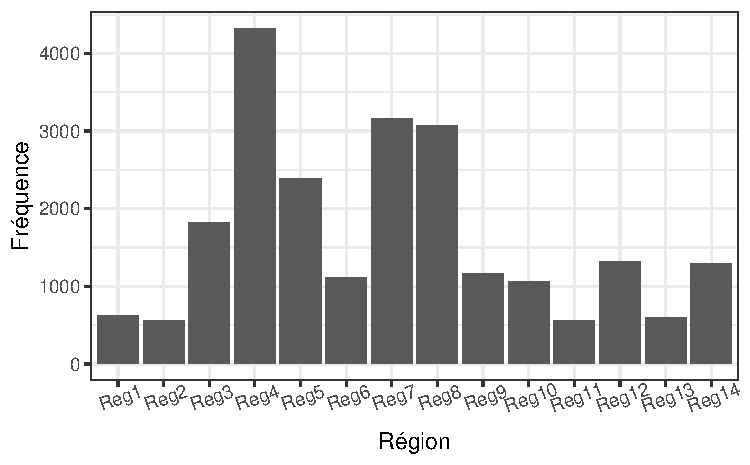
\includegraphics{01-01-Pretraitement_files/figure-latex/graph_vehicl_region-1} 

}

\caption{\label{fig:vehiclregion}Distribution des régions des détenteurs de police, représenté par la variable \textbf{polholder\_age}}\label{fig:graph_vehicl_region}
\end{figure}

Les assurés sont répartis dans toutes les régions on note toutefois que
la région 4 est la région pour laquelle il y a le plus d'assurés.

\hypertarget{variable-ordinal}{%
\subsection{Variable ordinal}\label{variable-ordinal}}

La variable catégorielle ordinale \textbf{prem\_freqperyear} représente
la fréquence par année à laquelle la prime est payable. Les fréquence
possible est mensuelle, trimestrielle, semestrielle ou annuelle.

\begin{figure}

{\centering 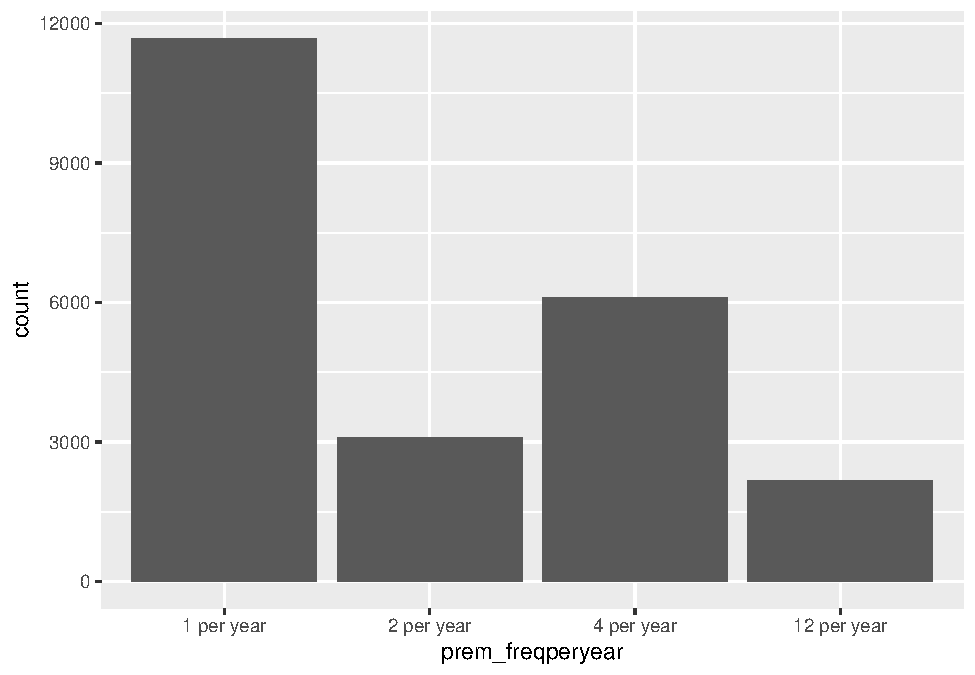
\includegraphics{01-01-Pretraitement_files/figure-latex/graph_prem_freqperyear-1} 

}

\caption{\label{fig:freqperyearAndvehiclGarage}todo}\label{fig:graph_prem_freqperyear}
\end{figure}

On voit qu'un peu moins de la moitié des clients paient la prime en un
seul versement, environ un quart des clients paient trimestriellement,
et le dernier quart est partagé par la prime payable semestriellement et
mensuellement.

La variable \textbf{vehicl\_powerkw} représente la puissance du moteur
de la voiture conduit exprimé en chevaux moteurs. Initialement, cette
variable contient 11 niveaux possibles. Cependant, en regardant les
niveaux, nous avons constaté que les données pour cette variable n'ont
pas été collectées uniformément puisque certaines catégories sont
comprises dans une autre catégorie. Un des niveaux correspond aux
véhicules d'une puissance se situant entre 125 et 300. Il y a aussi des
groupes pour lequels la puissance se trouve entre l'interval du groupe
présenté précédement, certains avec très peu d'observations d'autres
avec un peu plus d'observations. Or, puisqu'on ne sait pas la puissance
des voitures se trouvant dans le groupe de puissance 125-300 et que
celui-ci comprend un grand nombre d'observation nous avons opté pour
l'option d'ajouter les groupes pour lesquels leur puissance se situait
entre 125 et 300 chevaux. Pour facilité la représentation du traitement
effectué sur la variable \textbf{vehicl\_powerkw} voici un tableau de
fréquence avant traitement et tableau après traitement.

\begin{table}[!htb]
    \begin{minipage}{.5\linewidth}
      \caption{}
      \centering 
\begin{tabular}{cr}
\toprule
Puissance & Nombre d'observation\\
\midrule
100 kW & 5116\\
125-300 kW & 1720\\
150 kW & 580\\
175 kW & 206\\
200 kW & 32\\
\addlinespace
225 kW & 77\\
25-50 kW & 4968\\
250 kW & 16\\
275 kW & 4\\
300 kW & 2\\
\addlinespace
75 kW & 10339\\
\bottomrule
\end{tabular} \end{minipage}%
    \begin{minipage}{.5\linewidth}
      \centering
        \caption{} 
\begin{tabular}{cr}
\toprule
Puissance & Nombre d'observation\\
\midrule
25-50 kW & 4968\\
75 kW & 10339\\
100 kW & 5116\\
125-300 kW & 2637\\
\bottomrule
\end{tabular} \end{minipage} 
\end{table}

\hypertarget{variable-numuxe9rique}{%
\subsection{Variable numérique}\label{variable-numuxe9rique}}

La variable \textbf{polholder\_age} est une variable numérique discrète
représentant l'âge du propriétaire de la police d'assurance. La
\autoref{fig:polholderAge} représente la distribution de âges des
assurés.

\begin{figure}

{\centering 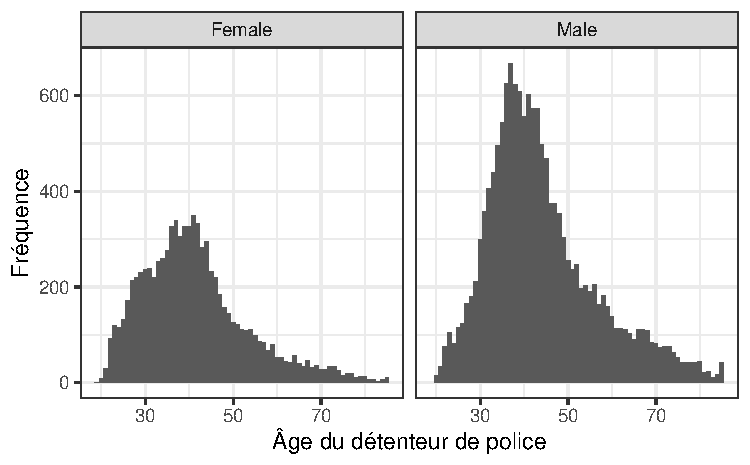
\includegraphics{01-01-Pretraitement_files/figure-latex/graph_polholder_age-1} 

}

\caption{\label{fig:polholderAge}Distribution de l'âge des détenteurs de polices dans la base de données, représenter par la variable \textbf{polholder\_age}}\label{fig:graph_polholder_age}
\end{figure}

L'âge minimal parmis les assuré est de 19 ans et l'âge maximal est de 85
ans. On constate qu'il y a une forte proportion d'assuré entre 30 et 45
ans. Il pourra être pertinent d'analyser si les assurés de plus de 45
ans sont présent en moins grand nombre dû au fait que les primes sont
trop élevé et font d'avantage d'appel pour comparer les primes ailleurs
ce qui les mènent vers la résignation.

Le nombre d'année sans résignation de la police d'assurance depuis la
première année assurée est représenté par la variable umérique discrète
\textbf{policy\_age}. Avec l'aide de la \autoref{fig:policyAge} on
constate une forte décroissance du nombre d'assurée pour le nombre
d'années depuis l'entré en vigueur pour les 3 premières années pour
ensuite ce stabilisé par la suite.

\begin{figure}

{\centering 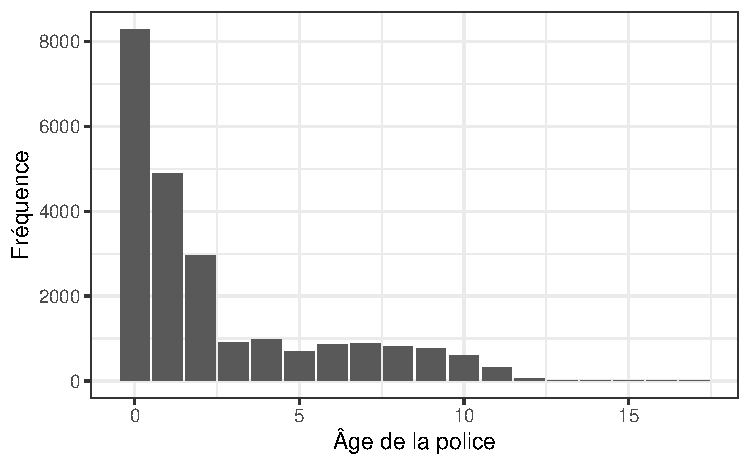
\includegraphics{01-01-Pretraitement_files/figure-latex/graph_policy_age-1} 

}

\caption{\label{fig:policyAge}Distribution de l'âge pour laquelle une police est en vigeur, représenter par la variable \textbf{policy\_age}}\label{fig:graph_policy_age}
\end{figure}

En ce qui concerne la variable discrète \textbf{policy\_nbcontract}
représentant le nombre de contrat, ou risque, que l'assuré possède chez
l'assureur. L'histogramme illustré à la \autoref{fig:policyNbcontract}
fait resortir le fait qu'il y a une forte concentration d'assuré pour
lesquels le nombre de contrat qu'ils ont chez l'assureur est inférieur à
5. On peut aussi voir que certains assurés ont jusqu'à 15 contrats.

\begin{figure}

{\centering 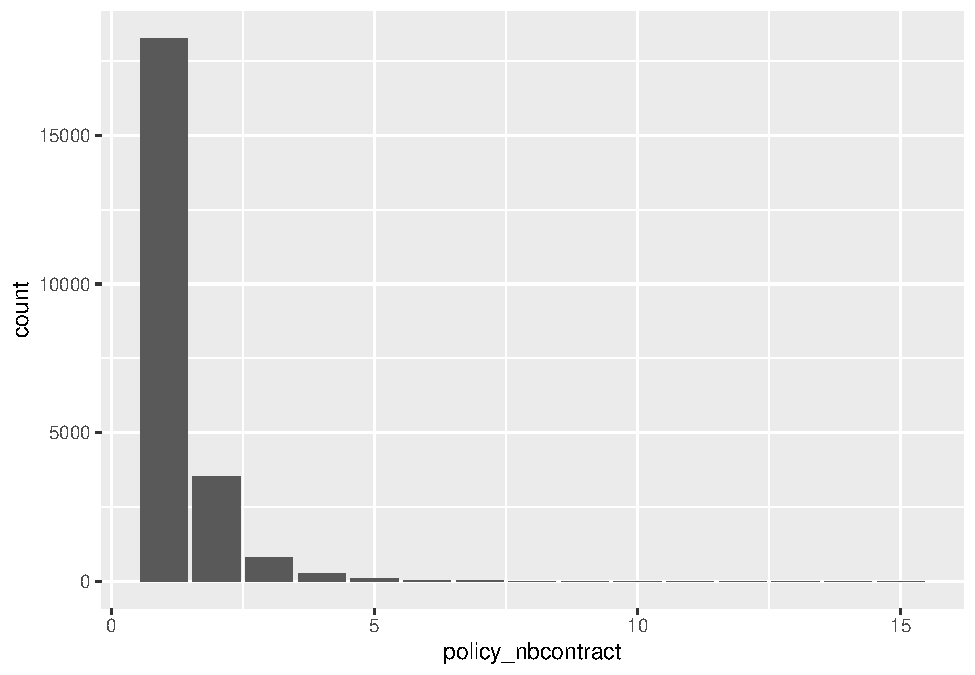
\includegraphics{01-01-Pretraitement_files/figure-latex/graph_policy_nbcontract-1} 

}

\caption{\label{fig:policyNbcontract}Distribution du nombre de contrats par police, représenter par la variable \textbf{policy\_nbcontract}}\label{fig:graph_policy_nbcontract}
\end{figure}

Il y a plusieurs variables numériques continues relatives à la prime. La
variable \textbf{prem\_final} représente le montant de la prime proposé
pour le renouvellement par l'assureur alors que \textbf{prem\_last}
représente le montant payé lors du dernier renouvellement. La variable
prem\_market est la prime qui serait chargée selon le marché. La
variable prem\_pure est la prime qui représente les coûts espérés pour
un assuré. Le \autoref{tbl:summaryPrimes} montre les distributions de
chaqune des primes. Par contre, une prime seul peut difficilement
expliquer pourquoi un assuré voudrais résigné car si l'assuré mérite
réellement sa prime, il n'aurait pas intérêt à aller chez un concurant.
Par contre, si lors de sont renouvellement, il voit sont montant
d'assurance augmenter d'un grand poucentage, il serat tenté d'aller voir
ayeur. C'est pourquoi la variable \textbf{prem\_index} à été crée et
ajouté à notre jeu de données. celle-ci représente le pourcentage
d'augmentation de la prime, sois la prime final divisé par la prime du
dernier terme.

\begin{table}[ht]
\centering
\caption{} 
\label{}
\begin{tabular}{lccccc}
  \hline
Prime (\$) & Minimum & Médiane & Moyenne & Maximum & Écart-type \\ 
  \hline
Final & 46.55 & 312.25 & 374.12 & 2948.05 & 212.9 \\ 
  Last & 46.56 & 311 & 380.51 & 3362.07 & 227.94 \\ 
  Market & 50.11 & 316.83 & 373.53 & 2416.84 & 201.92 \\ 
  Pure & 45.55 & 301.45 & 355.88 & 2716.08 & 197.14 \\ 
   \hline
Index (\%) & -0.58 & 0 & 0 & 2.27 & 0.1 \\ 
   \hline
\end{tabular}
\end{table}

Les deux prochaines variables sont en lien avec l'aĝe du véhicule, il
s'agit de variables numériques discrètes. La variable
vehicl\_agepurchase représente l'âge du véhicule lorsque l'assuré a
acheté le véhicule. La variable vehicl\_age représente l'aĝe du véhicule
actuellement.

\begin{figure}

{\centering 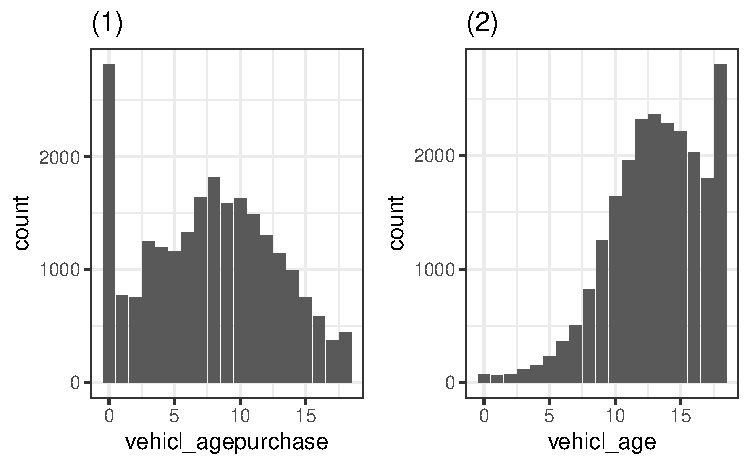
\includegraphics{01-01-Pretraitement_files/figure-latex/graph_age-1} 

}

\caption{\label{fig:}todo}\label{fig:graph_age}
\end{figure}

Beaucoup de véhicule ont été achetés lorsqu'il était neuf
(vehicl\_purchase = 0). En examinant les véhicules conduits par es
assurés on remarque qu'il y a peu de véhicule neuf et le nombre de
véhicule est croissant en fonction de l'utilisation jusqu'à 13 ans puis
décroit par la suite. On retrouve un grand nombre de véhicule assuré
avec 18 ans d'usage, il est fort probable que cela correspondre aux
véhicules de plus de 18 ans.

\newpage

\hypertarget{traitement-des-valeurs-manquantes}{%
\section{Traitement des valeurs
manquantes}\label{traitement-des-valeurs-manquantes}}

\newpage

\hypertarget{analyse-en-composantes-principales}{%
\section{Analyse en composantes
principales}\label{analyse-en-composantes-principales}}

Étant donné que notre jeu de données contient
\texttt{R\ nrow(Donnees\_tempo)} observations, il peut être utile de
visualiser les données à l'aide de l'analyse en composantes principales,
appelé ACP. En effet, ce type d'analyse permet de mieux visualiser un
jeu de données lorsque celui-ci est de grande dimension. Il sera ainsi
possible de voir quelles variables explicatives sont plus intéressantes
par leur impact sur la variance des composantes principales. Il est à
noter qu'en général, on garde assez de composantes pour représenter
entre 80 et 90 \% de la variance totale.

Pour que cette méthode de visualisation puisse être utilisée, il sera
nécessaire de prendre seulement les variables explicatives numériques de
ce jeu de donnée. Les variables catégorielles ne seront pas analysées
dans cette section car même en les transformant en variables numériques,
elles ne seront pas représentative des valeurs leur qui leur aurait été
attribuée en faisant la modification de type.

On doit ensuite choisir le nombre de composantes principales. Cette
étape peut être complétée en ayant deja un pourcentage de variance
expliquée en tête et en choisissant le nombre de composantes à partir
des valeurs propres ou en analysant directement le diagramme d'ébouli.
Dans ce cas, la méthode du coude ne sera pas utilisée, on priviligie
d'avantage le choix selon le premier plateau observée. Le nombre de
composantes choisit seront celle ne faisant pas partie du premier
plateau observée.

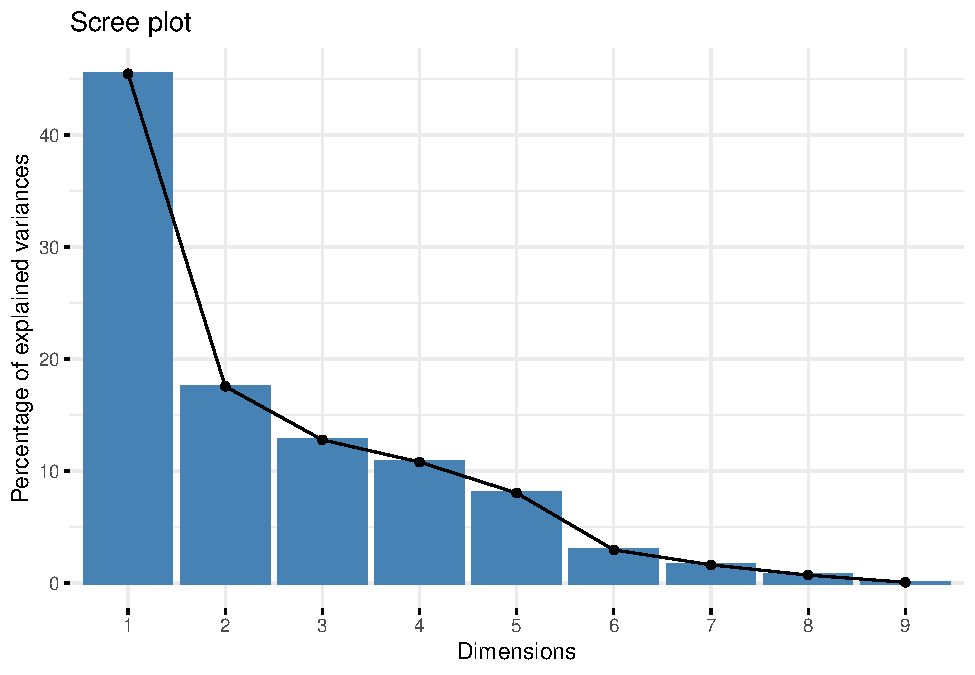
\includegraphics{01-01-Pretraitement_files/figure-latex/unnamed-chunk-3-1.pdf}

Selon le diagramme d'éboulis, il sera nécessaire de conserver 2
composantes principales et on observe, à l'aide des valeurs propres de
la matrice de corélation, que 2 composantes principales permettent
d'expliquer 63\% de la variance totale.

À l'aide du graphique ACP des variables, on peut voir la gravité des
contributions pour chacune des variables sur chaque composantes
principales retenu. Ainsi, on peut observer que pour la première
composante principale, un score élevé indique un contrat ayant une prime
élevée, que ce soit la prime du marché, la prime pure, la prime finale
ou la prime chargée lors du dernier renouvellement. Par contre, un
assuré âgé qui renouvelle depuis plusieurs année aura un score plus
faible qu'un assuré en bas âge ayant une police d'assurance récente. Un
score élevé représente donc un assuré en bas âge ayant une police
récente et une prime élevé tandis qu'un score faible représente une
personne plus âgée avec une faible prime d'assurance.

La deuxième composante principale représente, quant à elle, l'âge du
véhicule assuré. Un score élevé est associé à des véhicules de moindres
valeurs mais risquant d'avantage un bris de veillesse. Plus les polices
d'assurance sont récentes et plus le score en sera augmenté. Ainsi, les
polices d'assurances récente ayant des véhicules de l'année
représenteront les scores les plus faibles pour cette composante.

En illustrant les contributions des variables pour les deux premières
composantes principales, il est plus facile de visualiser les
conclusions mentionnées précédemment.

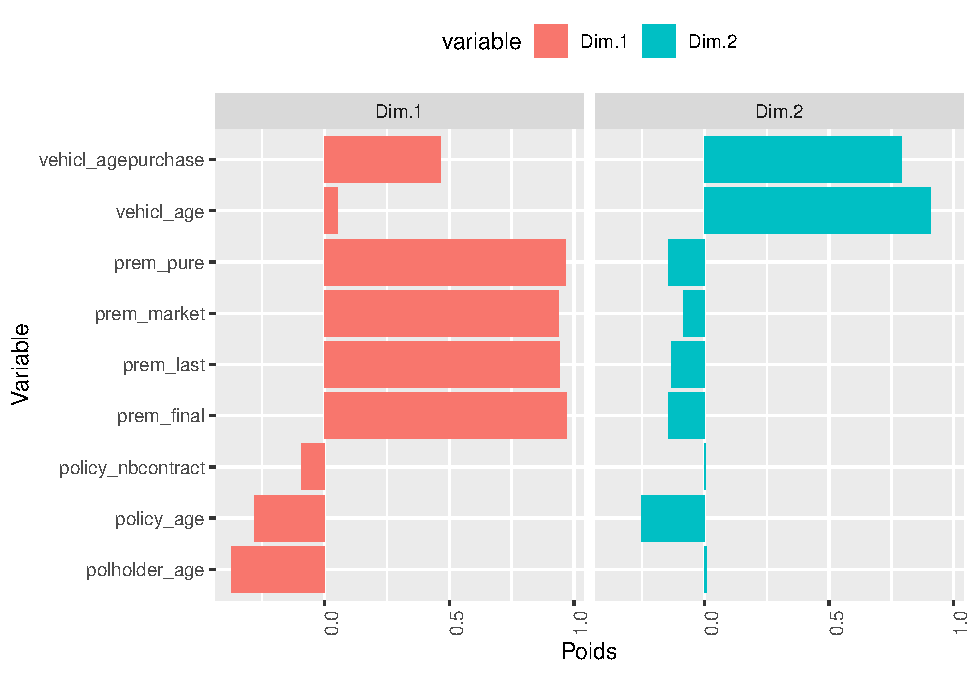
\includegraphics{01-01-Pretraitement_files/figure-latex/unnamed-chunk-5-1.pdf}

\newpage

\hypertarget{partitionnement-en-k-moyennes}{%
\section{Partitionnement en k
moyennes}\label{partitionnement-en-k-moyennes}}

Le partitionnement en k moyennes est utilisé pour classifier les
observations en k groupes distincts. La valeur de k est une valeur qu'on
transmet pour indiquer le nombre de partitions désirées. Chaque
observation sera ensuite assigné à un seul groupe. L'algorithme utilisée
pour ce type de partitionnement a pour objectif de minimiser la variance
intra-groupe.

Le choix du nombre de groupe peut être choisit à l'aide du diagramme
d'éboulis par la méthode du coude. Ainsi en ce réferant au graphique YYY
de la section ``Analyse en composantes principales'', on devrait faire
le partitionnement sur 6 groupes distincts. En effet le choix s'effectue
pour que le nombre de composantes apporte individuellement un
pourcentage de variance expliquée significatif. On s'arrête sur la
composante principale qui ce situe dans le ``pli de coude'', soit juste
avant le dernier plateau.

Voici le graphique obtenu pour le partitionnement en \(k\) moyennes :
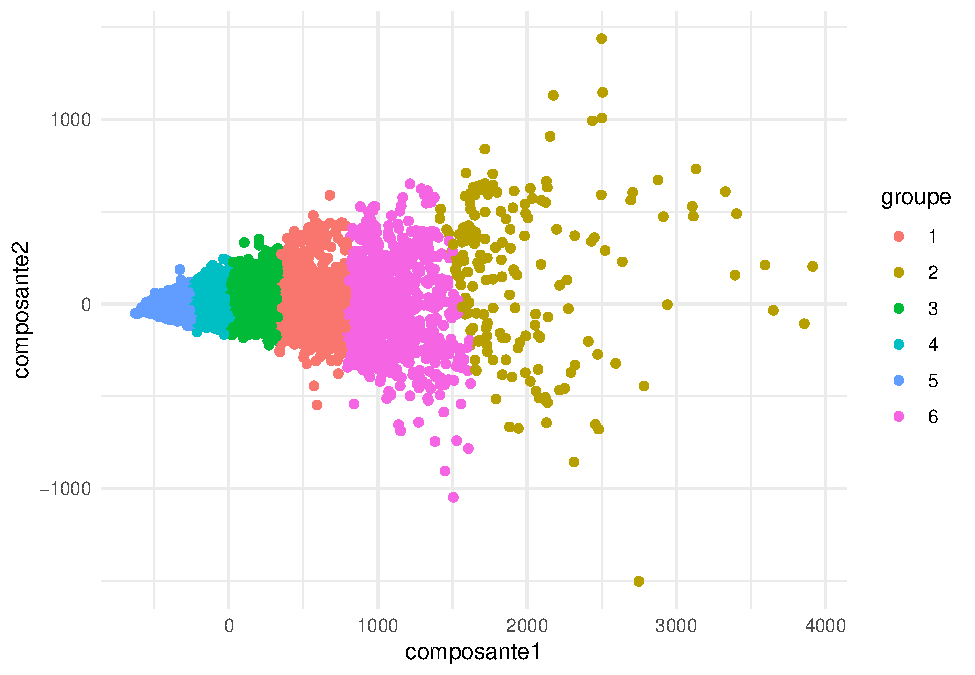
\includegraphics{01-01-Pretraitement_files/figure-latex/unnamed-chunk-6-1.pdf}

De ce graphique, on peut conclure que le partionnement c'est fait
vraiment que sur les montants des primes.

\newpage

\hypertarget{conclusion}{%
\section{Conclusion}\label{conclusion}}

\newpage

\hypertarget{bibliographie}{%
\section{Bibliographie}\label{bibliographie}}

\newpage

\hypertarget{annexe}{%
\section{Annexe}\label{annexe}}

Description du jeu de données soumis sur le forum :

Notre jeu de données représente le statut de renouvellement pour 23 060
polices d'assurance basées sur un an d'observation. Les données
receuillies proviennent d'une compagnie d'assurance inconnue dont
l'année d'observation est également inconnue.

\end{document}
